\chapter{अभिक्रिया की प्रगति सारणी}\label{ch:g10:reaction-progress-table}

% ledger: use:NaN3-airbag
कार दुर्घटना में स्टीयरिंग व्हील से एक गद्दी बाहर निकलती है और चालक का सिर आगे
बढ़ने से पहले, एक सेकंड के अंश में, गैस से भर जाती है। गैस एक \omterm{def:g7:chemical-reactions:reaction}{रासायनिक अभिक्रिया}
से बनती है: ठोस की एक छोटी मात्रा, पारंपरिक डिज़ाइन में सोडियम ऐज़ाइड, विघटित होकर
सोडियम और नाइट्रोजन बन जाती है। इंजीनियर को गद्दी भरने लायक ठोस डालना होता है,
पर इतना नहीं कि वह फट जाए, और कोई भी \omterm{def:g7:chemical-reactions:reactant}{अभिकारक} बचना नहीं चाहिए जो यात्रियों को
हानि पहुँचाए। कितना ठोस कितनी गैस देता है? \omterm{def:g8:balanced-equations:equation}{संतुलित समीकरण} अनुपात देता है;
यह अध्याय उन्हें हिसाब-किताब के एक औज़ार में बदलता है, जो किसी अभिक्रिया की
शुरुआत से अंत तक हर \omterm{def:g7:chemical-reactions:reactant}{अभिकारक} और हर उत्पाद पर नज़र
रखता है।

\begin{recall}
\omterm{def:g8:balanced-equations:equation}{संतुलित समीकरण} हर तत्व के \omterm{def:g7:atoms-and-molecules:atom}{परमाणुओं} की संख्या, और आवेश, दोनों ओर बराबर रखता है;
उसके गुणांक बताते हैं कि स्पीशीज़ किस अनुपात में अभिक्रिया करती हैं
(\cref{ch:g8:balanced-equations})। किसी स्पीशीज़ की मात्रा द्रव्यमान के लिए
$n = m/M$ है, गैस के लिए $n = V/V_m$ (\qty{20}{\celsius} और सामान्य
वायुमंडलीय दाब पर $V_m = \qty{24.1}{L/mol}$ के साथ)
(\cref{ch:g10:the-mole}), और \omterm{def:g6:solutions-and-solubility:solute}{विलेय} के लिए $n = c \times V$
(\cref{ch:g10:concentration-and-dilution})।
\end{recall}

\begin{omfigure}
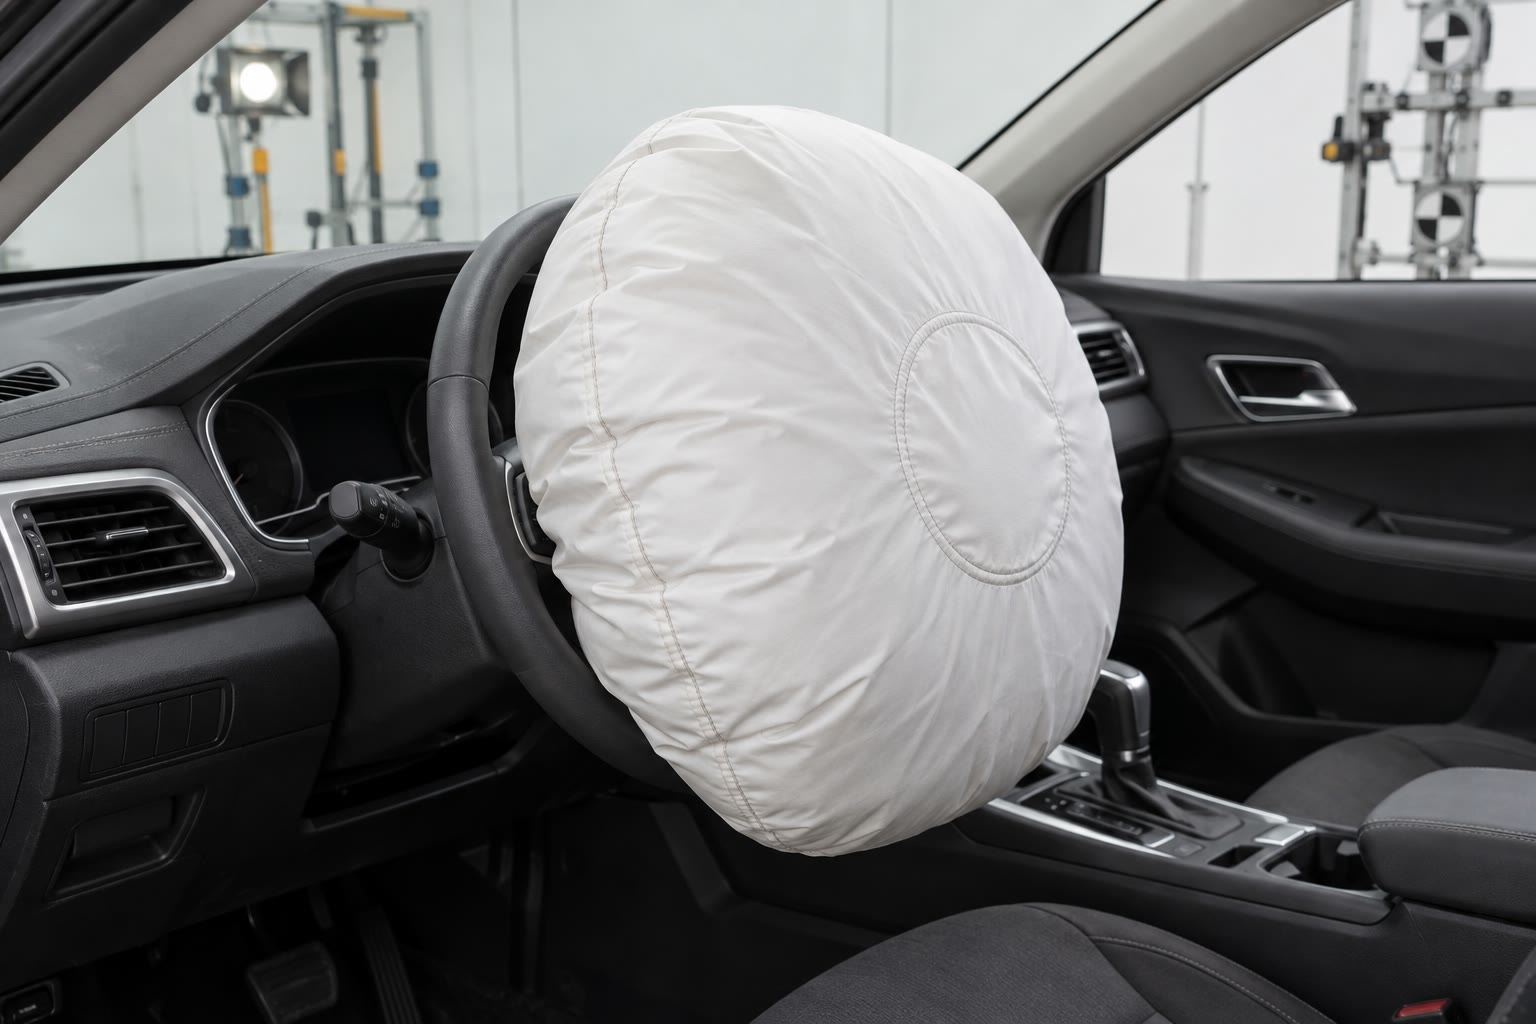
\includegraphics[width=0.5\linewidth]{images/book1/ai/g10-airbag.jpg}

{\small एयरबैग एक सेकंड के अंश में भर जाता है, एक अभिक्रिया से बनी
नाइट्रोजन से।}
\end{omfigure}

\section{रासायनिक निकाय का वर्णन}

\begin{definition}[रासायनिक निकाय, प्रारंभिक और अंतिम अवस्थाएँ]\label{def:g10:reaction-progress-table:system}
\emph{रासायनिक निकाय}\index{रासायनिक निकाय} किसी दिए गए स्थान (एक फ़्लास्क,
एक गद्दी, एक सेल) में मौजूद \omterm{def:g6:pure-substances-and-mixtures:species}{रासायनिक स्पीशीज़} का समूह है, हर एक अपनी मात्रा और
अपनी भौतिक अवस्था के साथ। अभिक्रिया शुरू होने से पहले का निकाय
\emph{प्रारंभिक अवस्था}\index{प्रारंभिक अवस्था} है; अभिक्रिया रुक जाने के बाद
का निकाय \emph{अंतिम
अवस्था}\index{अंतिम अवस्था} है।
\end{definition}


\begin{example}[बंद पात्र में मेथेन का जलना]\label{ex:g10:reaction-progress-table:methane}
एक बंद पात्र में \qty{2.0}{mol} मेथेन और \qty{3.0}{mol}
डाइऑक्सीजन है; एक चिंगारी \omterm{def:g4:what-a-fire-needs:burning}{दहन}
\ce{CH4 + 2O2 -> CO2 + 2H2O} शुरू कर देती है। \omterm{def:g10:reaction-progress-table:system}{प्रारंभिक अवस्था} में निकाय में
\qty{2.0}{mol} \ce{CH4(g)}, \qty{3.0}{mol} \ce{O2(g)} है और कोई
उत्पाद नहीं। \omterm{def:g10:reaction-progress-table:system}{अंतिम अवस्था} में क्या है? अध्याय का बाकी भाग इसका उत्तर देता है।
\end{example}

\section{अभिक्रिया की प्रगति और प्रगति सारणी}

\begin{definition}[अभिक्रिया की प्रगति, प्रगति सारणी]\label{def:g10:reaction-progress-table:extent}
\emph{अभिक्रिया की प्रगति}\index{अभिक्रिया की प्रगति} $x$, \omterm{def:g10:the-mole:amount}{मोल} में, गिनती है कि
\omterm{def:g8:balanced-equations:equation}{संतुलित समीकरण} में लिखी गई अभिक्रिया कितनी बार
हुई है: जब प्रगति $x$ है, तो गुणांक $\nu$ वाली किसी स्पीशीज़ की मात्रा
$\nu x$ खपत हुई है (\omterm{def:g7:chemical-reactions:reactant}{अभिकारक}) या बनी है (उत्पाद)।
\emph{प्रगति सारणी}\index{प्रगति सारणी} समीकरण के नीचे हर स्पीशीज़ की मात्रा
\omterm{def:g10:reaction-progress-table:system}{प्रारंभिक अवस्था} में, प्रगति $x$ पर, और \omterm{def:g10:reaction-progress-table:system}{अंतिम अवस्था} में
देती है।
\end{definition}

\begin{method}[प्रगति सारणी भरना]\label{met:g10:reaction-progress-table:fill}
\begin{enumerate}
  \item पहली पंक्ति में \omterm{def:g8:balanced-equations:equation}{संतुलित समीकरण} लिखिए।
  \item \omterm{def:g10:reaction-progress-table:system}{प्रारंभिक अवस्था} ($x = 0$): उसके नीचे हर स्पीशीज़ की प्रारंभिक मात्रा
        लिखिए।
  \item मध्यवर्ती अवस्था (प्रगति $x$): गुणांक $\nu$ वाला हर \omterm{def:g7:chemical-reactions:reactant}{अभिकारक}
        $n_0 - \nu x$ हो जाता है, हर उत्पाद $n_0 + \nu x$।
  \item \omterm{def:g10:reaction-progress-table:system}{अंतिम अवस्था}: $x_{\max}$ ज्ञात कीजिए (अगला खंड) और उसे मध्यवर्ती पंक्ति
        के व्यंजकों में रखिए।
\end{enumerate}
\end{method}

\begin{omfigure}
\renewcommand{\arraystretch}{1.25}
\begin{tabular}{l|c|cccc}
\hline
समीकरण & & \ce{CH4} & $+$ \ce{2O2} & $\longrightarrow$ \ce{CO2} & $+$ \ce{2H2O} \\
\hline
अवस्था & प्रगति (\si{mol}) & \multicolumn{4}{c}{मात्राएँ (\si{mol})} \\
\hline
प्रारंभिक & $0$ & $2.0$ & $3.0$ & $0$ & $0$ \\
मध्यवर्ती & $x$ & $2.0 - x$ & $3.0 - 2x$ & $x$ & $2x$ \\
अंतिम & $x_{\max} = 1.5$ & $0.5$ & $0$ & $1.5$ & $3.0$ \\
\hline
\end{tabular}\par\medskip

{\small उदाहरण के मेथेन \omterm{def:g4:what-a-fire-needs:burning}{दहन} की \omterm{def:g10:reaction-progress-table:extent}{प्रगति सारणी}।
हर स्तंभ एक स्पीशीज़ का अनुसरण करता है; \ce{O2} और
\ce{H2O} के गुणांक 2 ही $2x$ बनते हैं।}
\end{omfigure}

\section{सीमांत अभिकारक और अंतिम अवस्था}

\begin{definition}[सीमांत अभिकारक, अधिकतम प्रगति, पूर्ण अभिक्रिया]\label{def:g10:reaction-progress-table:limiting}
कोई अभिक्रिया \emph{पूर्ण अभिक्रिया}\index{पूर्ण अभिक्रिया} है अगर वह केवल तब रुकती
है जब उसका कोई एक \omterm{def:g7:chemical-reactions:reactant}{अभिकारक} पूरी तरह खप जाए। वह \omterm{def:g7:chemical-reactions:reactant}{अभिकारक}
\emph{सीमांत अभिकारक}\index{सीमांत अभिकारक} है; बाकी \omterm{def:g7:chemical-reactions:reactant}{अभिकारक}
आधिक्य में हैं। जिस प्रगति पर सीमांत \omterm{def:g7:chemical-reactions:reactant}{अभिकारक} ख़त्म होता है, वह
\emph{अधिकतम प्रगति}\index{अधिकतम प्रगति} $x_{\max}$ है; किसी पूर्ण अभिक्रिया की
\omterm{def:g10:reaction-progress-table:system}{अंतिम अवस्था} $x = x_{\max}$ वाली अवस्था है।
\end{definition}

\begin{method}[सीमांत अभिकारक ज्ञात करना]\label{met:g10:reaction-progress-table:limiting}
\begin{enumerate}
  \item हर \omterm{def:g7:chemical-reactions:reactant}{अभिकारक} के लिए $n_0 - \nu x = 0$ हल कीजिए: वह \omterm{def:g7:chemical-reactions:reactant}{अभिकारक}
        $x = n_0 / \nu$ पर ख़त्म होगा।
  \item इन मानों में सबसे छोटा $x_{\max}$ है; जो \omterm{def:g7:chemical-reactions:reactant}{अभिकारक} उसे देता है, वह
        \omterm{def:g10:reaction-progress-table:limiting}{सीमांत अभिकारक} है।
  \item \omterm{def:g10:reaction-progress-table:system}{अंतिम अवस्था} पाने के लिए $x_{\max}$ को मध्यवर्ती पंक्ति में रखिए;
        जाँचिए कि कोई मात्रा ऋणात्मक नहीं है।
\end{enumerate}
\end{method}

\begin{example}[मेथेन पर वापस]\label{ex:g10:reaction-progress-table:methane-final}
मेथेन $x = 2.0/1 = \qty{2.0}{mol}$ पर ख़त्म होगी, डाइऑक्सीजन
$x = 3.0/2 = \qty{1.5}{mol}$ पर। छोटा मान \qty{1.5}{mol} है: डाइऑक्सीजन
\omterm{def:g10:reaction-progress-table:limiting}{सीमांत अभिकारक} है और $x_{\max} = \qty{1.5}{mol}$। \omterm{def:g10:reaction-progress-table:system}{अंतिम अवस्था} में
\qty{0.5}{mol} मेथेन बची है, कोई डाइऑक्सीजन नहीं,
\qty{1.5}{mol} कार्बन डाइऑक्साइड और \qty{3.0}{mol} पानी है।
\end{example}

\begin{omfigure}
\begin{tikzpicture}
\begin{axis}[width=0.78\linewidth, height=6.2cm, xmin=0, xmax=2.05,
    ymin=0, ymax=4.2, xlabel={प्रगति $x$ (\si{mol})},
    ylabel={मात्रा (\si{mol})}, axis lines*=left, ymajorgrids,
    grid style={gray!20}, tick label style={font=\small},
    label style={font=\small}, xtick={0,0.5,1,1.5,2},
    legend style={font=\small, at={(1.02,0.5)}, anchor=west, draw=none},
    legend cell align=left]
  \addplot[very thick, omDef, domain=0:2] {2-x};
  \addplot[very thick, omThm, domain=0:1.5] {3-2*x};
  \addplot[very thick, omMeth, domain=0:2] {x};
  \addplot[very thick, omProp, domain=0:2] {2*x};
  \legend{\ce{CH4}, \ce{O2}, \ce{CO2}, \ce{H2O}}
  \addplot[dashed, black!60] coordinates {(1.5,0) (1.5,4.2)};
  \node[font=\small, anchor=south west] at (axis cs:1.5,3.55) {$x_{\max}$};
  \fill[black!8, opacity=0.6] (axis cs:1.5,0) rectangle (axis cs:2.05,4.2);
\end{axis}
\end{tikzpicture}

{\small मेथेन वाले उदाहरण के लिए प्रगति के विरुद्ध मात्राएँ। डाइऑक्सीजन
(लाल) सबसे पहले शून्य तक पहुँचती है, $x = \qty{1.5}{mol}$ पर: अभिक्रिया वहीं
रुक जाती है, और छायांकित भाग तक कभी नहीं पहुँचा जाता।}
\end{omfigure}

\begin{remark}[सभी अभिक्रियाएँ पूर्ण नहीं होतीं]\label{rem:g10:reaction-progress-table:not-total}
बहुत-सी अभिक्रियाएँ किसी \omterm{def:g7:chemical-reactions:reactant}{अभिकारक} के खपने से पहले ही रुक जाती हैं: वे ऐसी अवस्था
तक पहुँचती हैं जिसमें \omterm{def:g7:chemical-reactions:reactant}{अभिकारक} और उत्पाद साथ-साथ रहते हैं। उनकी \omterm{def:g10:reaction-progress-table:system}{अंतिम अवस्था}
$x_{\max}$ नहीं होती, और आगे का एक अध्याय उसे ज्ञात करना सिखाता है। इस अध्याय में
हर अभिक्रिया पूर्ण है।
\end{remark}

\section{रससमीकरणमितीय मिश्रण}

\begin{definition}[रससमीकरणमितीय मिश्रण]\label{def:g10:reaction-progress-table:stoichiometric}
\omterm{def:g7:chemical-reactions:reactant}{अभिकारकों} का \omterm{def:g6:pure-substances-and-mixtures:mixture}{मिश्रण} \emph{रससमीकरणमितीय
मिश्रण}\index{रससमीकरणमितीय मिश्रण} होता है जब प्रारंभिक मात्राएँ \omterm{def:g8:balanced-equations:equation}{संतुलित
समीकरण} के गुणांकों के अनुपात में हों।
\end{definition}

\begin{proposition}[सभी अभिकारक एक साथ ख़त्म होते हैं]\label{prop:g10:reaction-progress-table:together}
अभिक्रिया $a\,\ce{A} + b\,\ce{B} \longrightarrow$ उत्पाद के लिए \omterm{def:g6:pure-substances-and-mixtures:mixture}{मिश्रण}
रससमीकरणमितीय है यदि और केवल यदि
\[
  \frac{n_0(\ce{A})}{a} = \frac{n_0(\ce{B})}{b},
\]
और तब, \omterm{def:g10:reaction-progress-table:limiting}{पूर्ण अभिक्रिया} के लिए, \omterm{def:g10:reaction-progress-table:system}{अंतिम अवस्था} में दोनों \omterm{def:g7:chemical-reactions:reactant}{अभिकारक} खप जाते
हैं।
\end{proposition}

\begin{proof}
\ce{A} $x = n_0(\ce{A})/a$ पर ख़त्म होगा, \ce{B} $x = n_0(\ce{B})/b$ पर।
दोनों मान ठीक तभी बराबर होते हैं जब अनुपात समीकरण वाले हों, और तब
प्रगति $x_{\max}$ दोनों को एक साथ ख़ाली कर देती है।
\end{proof}

\begin{example}[मेथेन को साफ़-सुथरे ढंग से जलाना]\label{ex:g10:reaction-progress-table:stoich}
\ce{CH4 + 2O2 -> CO2 + 2H2O} के लिए \qty{2.0}{mol} मेथेन को
\qty{4.0}{mol} डाइऑक्सीजन चाहिए: $2.0/1 = 4.0/2$। केवल \qty{3.0}{mol}
डाइऑक्सीजन के साथ पहले उदाहरण के \omterm{def:g6:pure-substances-and-mixtures:mixture}{मिश्रण} में ऑक्सीजन कम थी; असली लौ में यही कमी
विषैली कार्बन मोनोऑक्साइड बनाती है
(\cref{ch:g8:combustion-and-fuels})।
\end{example}

\section{सारणी में गैसें और विलयन}


\begin{method}[प्रारंभिक अवस्था की मात्राएँ]\label{met:g10:reaction-progress-table:amounts}
सारणी भरने से पहले दी गई हर राशि को मात्रा में बदलिए:
तौले गए ठोस या द्रव के लिए $n = m/M$; गैस के लिए $n = V/V_m$;
घुली हुई स्पीशीज़ के लिए $n = c \times V$। अंत में \omterm{def:g10:reaction-progress-table:system}{अंतिम अवस्था} की मात्राओं को
वापस उसमें बदलिए जो पूछा गया हो: द्रव्यमान, गैस का आयतन या
सांद्रता।
\end{method}

\begin{example}[हाइड्रोक्लोरिक अम्ल में मैग्नीशियम]\label{ex:g10:reaction-progress-table:magnesium}
% ledger: aw:Mg
हाइड्रोक्लोरिक अम्ल में हाइड्रोजन \omterm{def:g9:ions:ion}{आयन} \ce{H+} होते हैं, जो मैग्नीशियम पर आक्रमण करते हैं:
\ce{Mg + 2H+ -> Mg^{2+} + H2}। \qty{0.12}{g} मैग्नीशियम का एक फ़ीता
$c(\ce{H+}) = \qty{1.0}{mol/L}$ वाले \qty{50.0}{mL} अम्ल में डाला जाता है।
प्रारंभिक मात्राएँ: $n_0(\ce{Mg}) = 0.12/24.3 = \qty{4.9e-3}{mol}$ और
$n_0(\ce{H+}) = 1.0 \times 0.0500 = \qty{5.0e-2}{mol}$। मैग्नीशियम
$x = \qty{4.9e-3}{mol}$ पर ख़त्म होगा, हाइड्रोजन \omterm{def:g9:ions:ion}{आयन}
$x = 0.050/2 = \qty{2.5e-2}{mol}$ पर: मैग्नीशियम सीमांत है और
$x_{\max} = \qty{4.9e-3}{mol}$। अभिक्रिया \qty{4.9e-3}{mol}
डाइहाइड्रोजन देती है, यानी \qty{20}{\celsius} पर $\num{4.9e-3} \times 24.1 = \qty{0.12}{L}$,
और $0.050 - 2 \times 0.0049 =
\qty{0.040}{mol}$ हाइड्रोजन \omterm{def:g9:ions:ion}{आयन} आधिक्य में छोड़ती है।
\end{example}

\begin{inthelab}[फ़्लास्कों पर गुब्बारे]
शिक्षक छह शंक्वाकार फ़्लास्कों में से हर एक में उसी हाइड्रोक्लोरिक अम्ल का
\qty{50.0}{mL} डालते हैं, और छह गुब्बारों में मैग्नीशियम चूर्ण के बढ़ते द्रव्यमान
रखते हैं: 0.15, 0.30, 0.45, 0.60, 0.75 और \qty{0.90}{g}। हर गुब्बारा
अपने फ़्लास्क की गर्दन पर चढ़ाया जाता है, फिर उठाया जाता है ताकि चूर्ण अम्ल में
गिर जाए। सनसनाते हुए गुब्बारे फूलते हैं। सब रुक जाने पर पहले से चौथे फ़्लास्क तक
गुब्बारे बड़े होते जाते हैं; चौथा, पाँचवाँ और छठा एक ही आकार के हैं, और आख़िरी
दो में फ़्लास्क की तली में कुछ धूसर चूर्ण बच जाता है।
\end{inthelab}

\begin{omfigure}
\begin{tikzpicture}[font=\small, scale=0.82]
  % H2 volume (L): 0.149 0.298 0.446 0.595 0.6025 0.6025; radius ~ V^(1/3)
  \foreach \i/\m/\v/\r/\left in {0/0.15/0.15/0.42/0, 1/0.30/0.30/0.53/0,
      2/0.45/0.45/0.61/0, 3/0.60/0.60/0.67/0, 4/0.75/0.60/0.67/1,
      5/0.90/0.60/0.67/1} {
    \begin{scope}[shift={(2.35*\i,0)}]
      \pic[transform shape] at (0,0) {erlenmeyer={0.25}{omWater}};
      \ifnum\left=1
        \fill[black!45] (-0.5,0.03) rectangle (0.5,0.12);
      \fi
      \fill[omProp!35, draw=omProp!80!black] (-0.3,2.6) -- (0.3,2.6)
        -- (0.12,2.82) -- (-0.12,2.82) -- cycle;
      \shade[ball color=omProp!40, draw=omProp!80!black]
        (0,{2.78+\r}) circle (\r);
      \node[align=center, anchor=north] at (0,-0.15)
        {\qty{\m}{g} Mg\\ \qty{\v}{L}};
    \end{scope}
  }
\end{tikzpicture}

{\small एक ही अम्ल और मैग्नीशियम के बढ़ते द्रव्यमानों वाले छह फ़्लास्क, हर गुब्बारे में
डाइहाइड्रोजन के आयतन (\qty{20}{\celsius} पर) के साथ।
लगभग \qty{0.61}{g} के बाद अम्ल सीमांत है: गुब्बारे बढ़ना बंद कर देते हैं
और मैग्नीशियम बच जाता है (धूसर)।}
\end{omfigure}

\begin{remark}[पठार को पढ़ना]\label{rem:g10:reaction-progress-table:plateau}
पहले फ़्लास्कों में मैग्नीशियम \omterm{def:g10:reaction-progress-table:limiting}{सीमांत अभिकारक} है, और उसे दुगना करने से गैस दुगनी
हो जाती है। एक निश्चित द्रव्यमान के बाद हाइड्रोजन \omterm{def:g9:ions:ion}{आयन} पहले ख़त्म होते हैं:
मैग्नीशियम मिलाने से बचे हुए चूर्ण के अलावा कुछ नहीं बदलता। यह बदलाव ठीक
\omterm{def:g10:reaction-progress-table:stoichiometric}{रससमीकरणमितीय मिश्रण} पर होता है,
$n_0(\ce{Mg}) = n_0(\ce{H+})/2 = \qty{0.025}{mol}$, यानी
$0.025 \times 24.3 = \qty{0.61}{g}$ मैग्नीशियम।
\end{remark}

\begin{safety}{\ghs[0.82cm]{GHS02}\ghs[0.82cm]{GHS05}\ghs[0.82cm]{GHS07}}
% ledger: ghs:Mg, ghs:HCl
मैग्नीशियम चूर्ण ज्वलनशील है; हाइड्रोक्लोरिक अम्ल त्वचा और आँखों को जलाता है
और उसके धुएँ श्वासमार्ग में जलन करते हैं; डाइहाइड्रोजन \omterm{def:g4:air-a-mixture-of-gases:air}{वायु} में \omterm{def:g4:what-a-fire-needs:burning}{जलती} है। यह
शिक्षक द्वारा किया गया प्रदर्शन है, चश्मा पहनकर, किसी भी लौ से दूर।
\end{safety}

\section{अभ्यास}

\begin{exercise}[$\star$]\label{exo:g10:reaction-progress-table:1}
\qty{4.0}{mol} डाइहाइड्रोजन और \qty{3.0}{mol} डाइऑक्सीजन के प्रारंभिक \omterm{def:g6:pure-substances-and-mixtures:mixture}{मिश्रण} के
लिए \ce{2H2 + O2 -> 2H2O} की \omterm{def:g10:reaction-progress-table:extent}{प्रगति सारणी} भरिए, यह मानकर कि
अभिक्रिया पूर्ण है। $x_{\max}$, \omterm{def:g10:reaction-progress-table:limiting}{सीमांत अभिकारक} और
\omterm{def:g10:reaction-progress-table:system}{अंतिम अवस्था} बताइए।
\end{exercise}

\begin{exercise}[$\star$]\label{exo:g10:reaction-progress-table:2}
कार्बन डाइऑक्सीजन में \omterm{def:g4:what-a-fire-needs:burning}{जलता} है: \ce{C + O2 -> CO2}। \qty{3.0}{mol}
कार्बन और \qty{2.0}{mol} डाइऑक्सीजन से शुरू करके $x_{\max}$, \omterm{def:g10:reaction-progress-table:limiting}{सीमांत
अभिकारक} और \omterm{def:g10:reaction-progress-table:system}{अंतिम अवस्था} ज्ञात कीजिए।
\end{exercise}

\begin{exercise}[$\star$]\label{exo:g10:reaction-progress-table:3}
गरम करने पर लोहा और सल्फ़र अभिक्रिया करते हैं: \ce{Fe + S -> FeS}।
\qty{0.50}{mol} लोहे और \qty{0.30}{mol} सल्फ़र से शुरू करके
\omterm{def:g10:reaction-progress-table:system}{अंतिम अवस्था} का वर्णन कीजिए।
\end{exercise}

\begin{exercise}[$\star$]\label{exo:g10:reaction-progress-table:4}
मान लीजिए अभिक्रिया \ce{N2 + 3H2 -> 2NH3} पूर्ण है।
\qty{1.0}{mol} डाइनाइट्रोजन और \qty{2.4}{mol} डाइहाइड्रोजन से शुरू करके
$x_{\max}$ और \omterm{def:g10:reaction-progress-table:system}{अंतिम अवस्था} ज्ञात कीजिए।
\end{exercise}

\begin{exercise}[$\star$]\label{exo:g10:reaction-progress-table:5}
\ce{2CO + O2 -> 2CO2} के लिए इनमें से कौन-सा \omterm{def:g6:pure-substances-and-mixtures:mixture}{मिश्रण} रससमीकरणमितीय है?
(क) \qty{2}{mol} \ce{CO} और \qty{2}{mol} \ce{O2}; (ख) \qty{4}{mol}
\ce{CO} और \qty{2}{mol} \ce{O2}; (ग) \qty{1}{mol} \ce{CO} और
\qty{2}{mol} \ce{O2}।
\end{exercise}

\begin{exercise}[$\star\star$]\label{exo:g10:reaction-progress-table:6}
\qty{32}{g} मेथेन को पूरी तरह \omterm{def:g4:what-a-fire-needs:burning}{जलाने} के लिए डाइऑक्सीजन का कितना द्रव्यमान चाहिए
(\ce{CH4 + 2O2 -> CO2 + 2H2O})? पानी का कितना द्रव्यमान बनता है?
\end{exercise}

\begin{exercise}[$\star\star$]\label{exo:g10:reaction-progress-table:7}
एक कैंपिंग स्टोव \qty{1.0}{kg} प्रोपेन जलाता है:
\ce{C3H8 + 5O2 -> 3CO2 + 4H2O}। वह \qty{20}{\celsius} पर कार्बन डाइऑक्साइड
का कितना आयतन छोड़ता है?
\end{exercise}

\begin{exercise}[$\star\star$]\label{exo:g10:reaction-progress-table:8}
मेथेन वाले उदाहरण के लिए प्रगति के विरुद्ध मात्राओं वाले चित्र की मदद से
$x = \qty{1.0}{mol}$ पर चारों स्पीशीज़ की मात्राएँ पढ़िए।
डाइऑक्सीजन की रेखा $x = \qty{1.5}{mol}$ पर क्यों रुक जाती है?
\end{exercise}

\begin{exercise}[$\star\star$]\label{exo:g10:reaction-progress-table:9}
\qty{0.10}{mol/L} वाले नीले कॉपर सल्फ़ेट विलयन के \qty{100.0}{mL} में
\qty{1.30}{g} ज़िंक चूर्ण मिलाया जाता है। अभिक्रिया है
\ce{Zn + Cu^{2+} -> Zn^{2+} + Cu}।
\omterm{def:g10:reaction-progress-table:limiting}{सीमांत अभिकारक}, बनने वाले ताँबे का द्रव्यमान और बचे हुए ज़िंक का द्रव्यमान ज्ञात
कीजिए। क्या अंत में विलयन अब भी नीला है?
\end{exercise}

\begin{exercise}[$\star\star$]\label{exo:g10:reaction-progress-table:10}
$c(\ce{H+}) = \qty{1.0}{mol/L}$ वाले \qty{20.0}{mL} हाइड्रोक्लोरिक अम्ल में
\qty{0.48}{g} मैग्नीशियम मिलाया जाता है
(\ce{Mg + 2H+ -> Mg^{2+} + H2})। कौन-सा \omterm{def:g7:chemical-reactions:reactant}{अभिकारक} सीमांत है? \qty{20}{\celsius}
पर डाइहाइड्रोजन का कितना आयतन इकट्ठा होता है?
\end{exercise}

\begin{exercise}[$\star\star$]\label{exo:g10:reaction-progress-table:11}
अभ्यास~3 में आधिक्य वाला \omterm{def:g7:chemical-reactions:reactant}{अभिकारक}, \omterm{def:g10:reaction-progress-table:stoichiometric}{रससमीकरणमितीय मिश्रण} बनाने वाली मात्रा से
कितने प्रतिशत अधिक है?
\end{exercise}

\begin{exercise}[$\star\star\star$]\label{exo:g10:reaction-progress-table:12}
एक छात्र \ce{Fe + S -> FeS} के लिए लोहे और सल्फ़र का \qty{10.0}{g}
\omterm{def:g10:reaction-progress-table:stoichiometric}{रससमीकरणमितीय मिश्रण} चाहता है। लोहे और सल्फ़र के कितने द्रव्यमान
तौलने होंगे?
\end{exercise}

\begin{exercise}[$\star\star\star$]\label{exo:g10:reaction-progress-table:13}
\qty{10.0}{g} चूना पत्थर \ce{CaCO3} को तेज़ गरम किया जाता है और वह पूरी तरह
विघटित हो जाता है: \ce{CaCO3 -> CaO + CO2}। मिले हुए बिना बुझे चूने \ce{CaO} को फिर
\qty{1.8}{g} पानी में डाला जाता है: \ce{CaO + H2O -> Ca(OH)2}।
\begin{enumerate}
  \item पहली \omterm{def:g10:reaction-progress-table:extent}{अभिक्रिया की प्रगति} सारणी भरिए; \qty{20}{\celsius} पर कार्बन
        डाइऑक्साइड का कितना आयतन निकलता है?
  \item दूसरी अभिक्रिया की सारणी भरिए। कौन-सा \omterm{def:g7:chemical-reactions:reactant}{अभिकारक}
        सीमांत है? बुझे चूने \ce{Ca(OH)2} का कितना द्रव्यमान बनता है?
\end{enumerate}
\end{exercise}

\begin{exercise}[$\star\star\star$]\label{exo:g10:reaction-progress-table:14}
प्रयोगशाला-खाने वाले गुब्बारा प्रयोग में हर गुब्बारे में डाइहाइड्रोजन का आयतन
निकालिए। समझाइए कि चौथे फ़्लास्क के बाद वह बढ़ना क्यों बंद कर देता है, और
मैग्नीशियम के द्रव्यमान के विरुद्ध गैस का आयतन (हाथ से) आलेखित
कीजिए।
\end{exercise}

\begin{exercise}[$\star\star\star$]\label{exo:g10:reaction-progress-table:15}
\qty{20}{\celsius} पर \qty{4.8}{L} डाइऑक्सीजन वाले एक बंद पात्र में \qty{4.6}{g}
एथेनॉल \ce{C2H6O} \omterm{def:g4:what-a-fire-needs:burning}{जलता} है:
\ce{C2H6O + 3O2 -> 2CO2 + 3H2O}। \omterm{def:g10:reaction-progress-table:limiting}{सीमांत अभिकारक}, बिना जले एथेनॉल का
द्रव्यमान और बनी कार्बन डाइऑक्साइड का आयतन ज्ञात कीजिए।
\end{exercise}

\section{समस्या: एयरबैग}

\begin{problem}[{सप्ताहांत समस्या --- 60 लीटर के एयरबैग को भरने के लिए स्टीयरिंग
व्हील में सोडियम ऐज़ाइड का कितना द्रव्यमान भरना होगा?}]
\label{pb:g10:reaction-progress-table:1}
% ledger: use:NaN3-airbag, ghs:NaN3, aw:Na, aw:N, aw:K, aw:O
पारंपरिक एयरबैग डिज़ाइन में बिजली की एक चिंगारी ठोस सोडियम ऐज़ाइड का
विघटन शुरू कर देती है:
\[
  \ce{2NaN3 -> 2Na + 3N2} .
\]
बनने वाली सोडियम \omterm{def:g9:periodic-table-first-look:metal}{धातु} ख़तरनाक है: वह पानी के साथ, और त्वचा और आँखों की नमी के
साथ, तीव्र अभिक्रिया करती है। इसलिए भरे गए \omterm{def:g6:pure-substances-and-mixtures:mixture}{मिश्रण} में पोटैशियम नाइट्रेट भी होता है, जो
सोडियम को हानिरहित ऑक्साइडों में बदल देता है और थोड़ी और नाइट्रोजन
देता है:
\[
  \ce{10Na + 2KNO3 -> K2O + 5Na2O + N2} .
\]
दोनों अभिक्रियाएँ पूर्ण हैं। एयरबैग को \qty{60}{L}
नाइट्रोजन से भरना है; गैस को \qty{20}{\celsius} पर लीजिए, जहाँ
$V_m = \qty{24.1}{L/mol}$।

\medskip
\noindent\textbf{भाग I --- अभिक्रियाएँ।}
\begin{enumerate}
  \item तत्व-दर-तत्व जाँचिए कि पहला समीकरण संतुलित है।
  \item जाँचिए कि दूसरा समीकरण संतुलित है।
  \item किस पिछले अध्याय ने दिखाया कि सोडियम पानी के साथ तीव्र अभिक्रिया करता
        है? दुर्घटना के बाद कोई सोडियम क्यों नहीं बचना चाहिए?
  \item सोडियम ऐज़ाइड \ce{NaN3} और
        पोटैशियम नाइट्रेट \ce{KNO3} के \omterm{def:g10:the-mole:molar-mass}{मोलर द्रव्यमान} निकालिए।
\end{enumerate}

\medskip
\noindent\textbf{भाग II --- विघटन।}
\begin{enumerate}[resume]
  \item सोडियम ऐज़ाइड की \qty{1.00}{mol} प्रारंभिक मात्रा के लिए पहली
        \omterm{def:g10:reaction-progress-table:extent}{अभिक्रिया की प्रगति} सारणी भरिए।
  \item $x_{\max}$ ज्ञात कीजिए। \omterm{def:g10:reaction-progress-table:limiting}{सीमांत अभिकारक} कौन-सा है?
  \item \omterm{def:g10:reaction-progress-table:system}{अंतिम अवस्था} में सोडियम और नाइट्रोजन की मात्राएँ बताइए।
  \item \qty{1.00}{mol} सोडियम ऐज़ाइड \qty{20}{\celsius} पर नाइट्रोजन का कितना
        आयतन देता है?
\end{enumerate}

\medskip
\noindent\textbf{भाग III --- सोडियम को हटाना।}
\begin{enumerate}[resume]
  \item दूसरी \omterm{def:g10:reaction-progress-table:extent}{अभिक्रिया की प्रगति} सारणी भरिए, प्रश्न 7 में मिले सोडियम
        और पोटैशियम नाइट्रेट की मात्रा $n$ से
        शुरू करके।
  \item पोटैशियम नाइट्रेट की कितनी मात्रा, और कितना द्रव्यमान, इस सोडियम के साथ
        \omterm{def:g10:reaction-progress-table:stoichiometric}{रससमीकरणमितीय मिश्रण} बनाता है?
  \item इस \omterm{def:g6:pure-substances-and-mixtures:mixture}{मिश्रण} के लिए दूसरी अभिक्रिया की \omterm{def:g10:reaction-progress-table:system}{अंतिम अवस्था} बताइए।
  \item अगर केवल \qty{0.150}{mol} पोटैशियम नाइट्रेट डाला जाता, तो कौन-सा
        \omterm{def:g7:chemical-reactions:reactant}{अभिकारक} सीमांत होता, और क्या बचता? यह ख़तरनाक क्यों
        होता?
\end{enumerate}

\medskip
\noindent\textbf{भाग IV --- 60 लीटर की थैली।}
\begin{enumerate}[resume]
  \item प्रश्न 7 और 11 से बताइए कि पूरा \omterm{def:g6:pure-substances-and-mixtures:mixture}{मिश्रण} सोडियम ऐज़ाइड के प्रति \omterm{def:g10:the-mole:amount}{मोल}
        नाइट्रोजन की कितनी मात्रा देता है?
  \item थैली को नाइट्रोजन की कितनी मात्रा भरती है?
  \item आवश्यक सोडियम ऐज़ाइड की मात्रा निकालिए।
  \item उसका द्रव्यमान निकालिए।
  \item मिलाए जाने वाले पोटैशियम नाइट्रेट का द्रव्यमान निकालिए।
  \item दूसरी अभिक्रिया के बिना सोडियम ऐज़ाइड का कितना द्रव्यमान चाहिए
        होता? दूसरी अभिक्रिया कितनी बचत करती है?
  \item सोडियम ऐज़ाइड निगलने पर घातक है। पहली अभिक्रिया का पूर्ण होना
        क्यों महत्वपूर्ण है, और \omterm{def:g10:reaction-progress-table:extent}{प्रगति सारणी} कैसे दिखाती है कि उसमें से कुछ
        नहीं बचता?
  \item अंतिम उत्तर बताइए: सोडियम ऐज़ाइड का कितना द्रव्यमान
        \qty{60}{L} का एयरबैग भरता है?
\end{enumerate}
\end{problem}
